\documentclass[12pt]{dforeport}
\usepackage{fancyhdr}
\usepackage{hanging}
\usepackage{lastpage}
\usepackage{setspace}
\usepackage{graphicx}
\usepackage{rotating}
\usepackage{times}
\usepackage{amsmath}
\usepackage{color}
\usepackage{tabularx}
\usepackage{natbib}
\usepackage{Sweave}
\usepackage[T1]{fontenc}
\usepackage{hyperref}
\usepackage{float}

% bib punctuation
\bibpunct{(}{)}{;}{a}{,}{,}

%\title{Chlorophyll Bloom Fitting Methods}
\title{(Insert title here)}
\author{(Insert author name(s) here)} % example : John Doe
\authorshort{(Insert abbreviated author name(s) here)} % example : Doe, J.
\year{(Insert year here)}
\reportnum{xxxx}
\catno{Fs 97-18} %shouldn't change
\issnprint{0711-6764} %shouldn't change
\issnelectronic{1488-5417} %shouldn't change

\begin{document}
\frontmatter
\mainmatter
\spacing{1.25} % 1.25 line spacing for document does not affect title and toc
\fontsize{10}{12}\selectfont
\section{Introduction}

Here are some references that I stole from the oce thesis example, \cite{Baines1982}, \cite{Voss2001}, \cite{Baines1973}.


Lorem ipsum dolor sit amet, consectetur adipiscing elit. Donec nibh est, efficitur vitae luctus sed, suscipit id magna. Ut non quam accumsan justo vulputate feugiat eget sit amet arcu. Nulla blandit lacinia erat, a lobortis est auctor quis. Etiam at dui pharetra, feugiat sem sit amet, bibendum nunc. Maecenas tincidunt lorem vel metus auctor cursus. Mauris suscipit suscipit diam, pharetra vulputate ex finibus in. Fusce cursus dictum nisl, in molestie ligula placerat eu. Praesent vestibulum purus ac pulvinar dapibus. Nam ornare, nisi a dapibus ultricies, nunc ipsum eleifend leo, sed euismod dui mi ut risus. Fusce eleifend enim eget semper posuere. Etiam mollis odio ac iaculis viverra. Pellentesque habitant morbi tristique senectus et netus et malesuada fames ac turpis egestas.

\subsection{Intro subsection}
Lorem ipsum dolor sit amet, consectetur adipiscing elit. Donec nibh est, efficitur vitae luctus sed, suscipit id magna. Ut non quam accumsan justo vulputate feugiat eget sit amet arcu. Nulla blandit lacinia erat, a lobortis est auctor quis. Etiam at dui pharetra, feugiat sem sit amet, bibendum nunc. Maecenas tincidunt lorem vel metus auctor cursus. Mauris suscipit suscipit diam, pharetra vulputate ex finibus in. Fusce cursus dictum nisl, in molestie ligula placerat eu. Praesent vestibulum purus ac pulvinar dapibus. Nam ornare, nisi a dapibus ultricies, nunc ipsum eleifend leo, sed euismod dui mi ut risus. Fusce eleifend enim eget semper posuere. Etiam mollis odio ac iaculis viverra. Pellentesque habitant morbi tristique senectus et netus et malesuada fames ac turpis egestas.

\subsubsection{Subsubsection}
An example of a sub sub section.


\section{Data}
Lorem ipsum dolor sit amet, consectetur adipiscing elit. Donec nibh est, efficitur vitae luctus sed, suscipit id magna. Ut non quam accumsan justo vulputate feugiat eget sit amet arcu. Nulla blandit lacinia erat, a lobortis est auctor quis. Etiam at dui pharetra, feugiat sem sit amet, bibendum nunc. Maecenas tincidunt lorem vel metus auctor cursus. Mauris suscipit suscipit diam, pharetra vulputate ex finibus in.


\begin{equation}
y = x^2
\label{e:squareFn}
\end{equation}

Lorem ipsum dolor sit amet, consectetur adipiscing elit. Donec nibh est, efficitur vitae luctus sed, suscipit id magna. Ut non quam accumsan justo vulputate feugiat eget sit amet arcu. Nulla blandit lacinia erat, a lobortis est auctor quis. Etiam at dui pharetra, feugiat sem sit amet, bibendum nunc. Maecenas tincidunt lorem vel metus auctor cursus. Mauris suscipit suscipit diam, pharetra vulputate ex finibus in.


\begin{table}
  \begin{center}
  \label{t:results}
    \begin{tabular}{|l|l|}
      \hline
      x  & y\\
      \hline
      1  & 1\\
      2 & 4\\
      \hline
    \end{tabular}
  \end{center}
  \caption[Results of Equation \eqref{e:squareFn}.]{Results of Equation \eqref{e:squareFn} with some extra text in the caption to show the difference between the TOC caption and in-text caption.}
\end{table}

Lorem ipsum dolor sit amet, consectetur adipiscing elit. Donec nibh est, efficitur vitae luctus sed, suscipit id magna. Ut non quam accumsan justo vulputate feugiat eget sit amet arcu. Nulla blandit lacinia erat, a lobortis est auctor quis. Etiam at dui pharetra, feugiat sem sit amet, bibendum nunc. Maecenas tincidunt lorem vel metus auctor cursus. Mauris suscipit suscipit diam, pharetra vulputate ex finibus in.

\begin{figure}
\centering
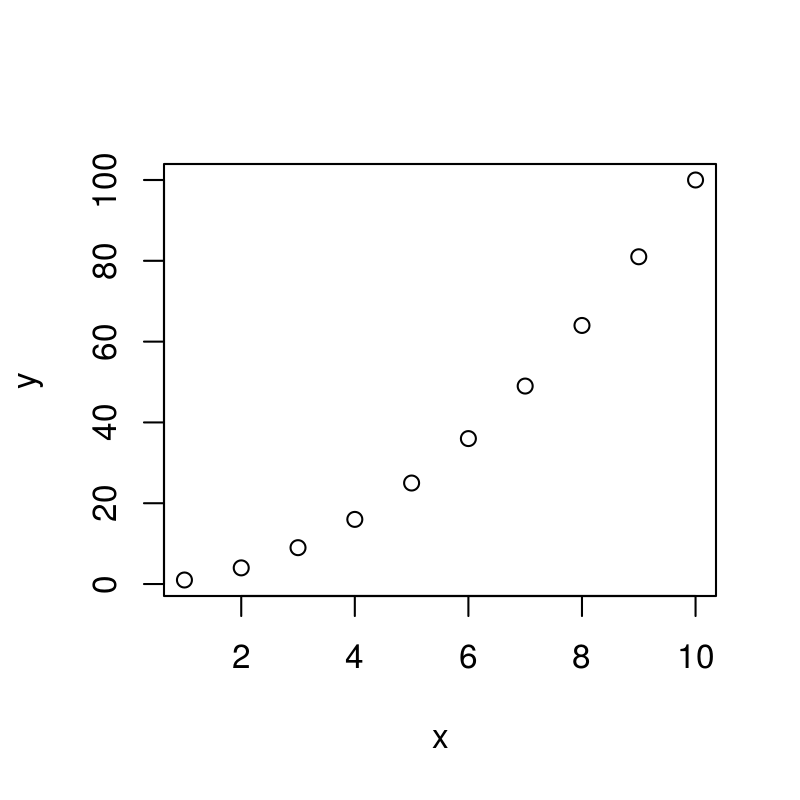
\includegraphics[width = 0.8\textwidth]{01_exampleFigure.png}
\caption[Plot of Equation \eqref{e:squareFn}]{A plot of Equation \eqref{e:squareFn} with some extra text in the caption to drive home the importance of the latex feature that so many people ignore.}
\label{f:results}
\end{figure}

Here is an example of citing Table \ref{t:results}, and Figure \ref{f:results}.

\section{Discussion}

Lorem ipsum dolor sit amet, consectetur adipiscing elit. Donec nibh est, efficitur vitae luctus sed, suscipit id magna. Ut non quam accumsan justo vulputate feugiat eget sit amet arcu. Nulla blandit lacinia erat, a lobortis est auctor quis. Etiam at dui pharetra, feugiat sem sit amet, bibendum nunc. Maecenas tincidunt lorem vel metus auctor cursus. Mauris suscipit suscipit diam, pharetra vulputate ex finibus in.

\pagebreak
\bibliographystyle{plainnat}
\bibliography{references}



\end{document}

